
\chapter{Project Overview}\label{section:introduction}
\thispagestyle{pagestyle}


The Messenger Application is a real-time chat platform designed to facilitate seamless communication between users through instant messaging and multimedia sharing. The application allows users to send and receive messages in one-on-one and group chats, manage their contacts, and personalize their profiles. To ensure a safe and organized environment, administrators have the ability to moderate content, manage users, and review reports.


The primary objective of this project is to develop a scalable, efficient, and user-friendly messenger software designe that supports real-time communication while ensuring security, privacy, and moderation. The designe will be build with an event-driven architecture using the Observer Pattern to handle real-time message delivery.



When designing a Messenger Application, or any software system, it is essential to create structured diagrams to visualize, analyze, and document the system before development. In this scope wee use Use Case Diagrams, UML Class Diagrams and Sequence Diagrams.


A Use Case Diagram is a behavioral diagram used in software engineering to visually represent the interactions between users (actors) and the system. It focuses on what the system does from the user’s perspective, rather than how it does it. Use Case Diagrams are part of the Unified Modeling Language (UML) and are widely used in the design phase of software development to understand the system's functional requirements. A Use Case Diagram is used to capture Functional Requirements. It identifies the key functions the system must perform. We can understand User Interaction and help developers and stakeholders understand how different users will interact with the system. The diagram provides a High-Level View, a simplified, visual overview of the system's major functionalities. IT facilitates communication by ensuring that all stakeholders (developers, business analysts, designers, etc.) are aligned on the system’s objectives.

A UML Class Diagram is a structural diagram in the Unified Modeling Language (UML) that represents the static structure of a system by modeling its classes, attributes, operations, and relationships. It is widely used in software engineering to visualize, specify, and document the architecture of a system.







A Sequence Diagram illustrates how objects interact over time during a specific use case, focusing on message flow between components.



\chapter{UML Use Case diagram}
\thispagestyle{pagestyle}
A Use Case Diagram represents the functional requirements of the system. It shows how users (actors) interact with the system’s functionalities (use cases).

\begin{figure}[h]
    \centering
    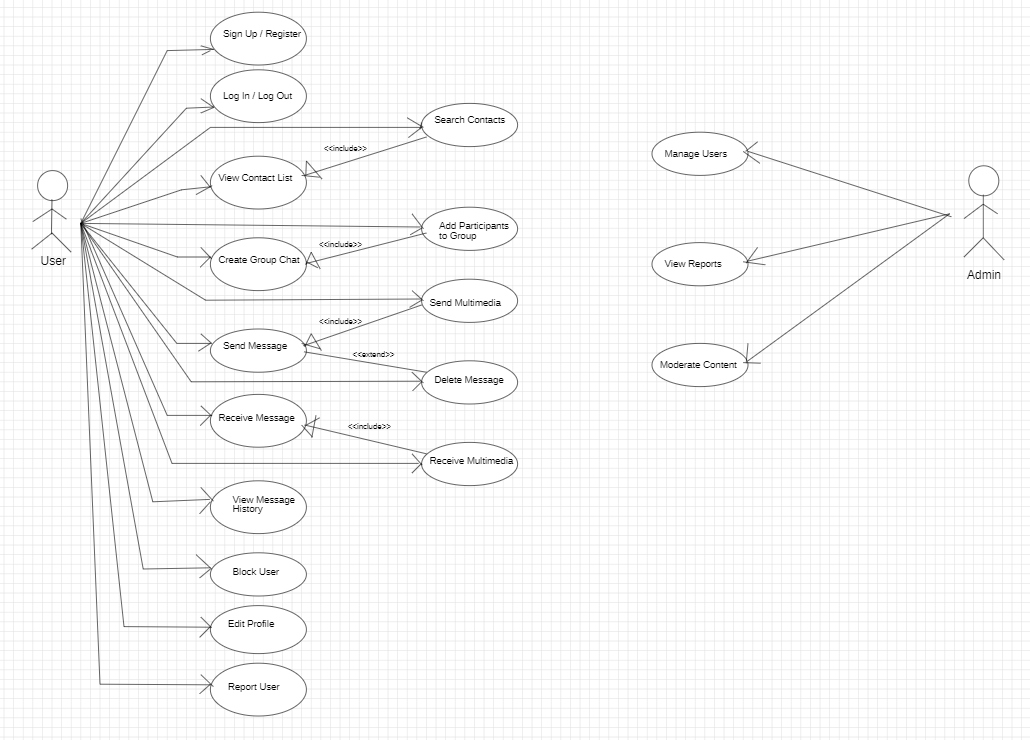
\includegraphics[width=1\textwidth]{images/use_case.png} % Adjust width as needed
    \caption{UML Use case diagram}
    \label{fig:example}
\end{figure}

This application is designed to offer a seamless messaging experience with an intuitive interface, ensuring users can engage efficiently. It is structured with two primary roles:
\begin{enumerate}
    \item User: A standard user who can send and receive messages, manage contacts, and customize their profile.
    \item Admin: An administrator responsible for managing users, handling reports, and moderating content.
\end{enumerate}

User Use cases: 
\begin{enumerate}
    \item Sign Up / Register: A user can create a new account by providing necessary details like email, username, and password.
    \item Log In / Log Out: Allows users to log into their account using valid credentials and log out when finished.
    \item View Contact List: The user can see a list of their saved contacts.
    \item Search Contacts (Included in View Contact List): Users can search for other people using their username or other identifiers.
    \item Create Group Chat: Users can create a group chat by adding multiple participants.
    \item Add Participants to Group (Included in Create Group Chat): Users can invite additional members to an existing group chat.
    \item Send Message: Users can send text messages to individual contacts or group chats.
    \item Send Multimedia (Included in Send Message): Users can send multimedia files such as images, videos, and audio messages.
    \item Delete Message (Extends Send Message): A user can delete a previously sent message.
    \item Receive Message: Users receive incoming messages from contacts.
    \item Receive Multimedia (Included in Receive Message): Users can receive and view multimedia messages.
    \item View Message History: Users can browse their past conversations.
    \item Block User: Users can block another user to prevent further communication.
    \item Edit Profile: Users can update their profile details, including username, profile picture, and bio.
    \item Report User: Users can report another user for inappropriate behavior or violations.    
\end{enumerate}

Admin Use Cases: 
\begin{enumerate}
    \item Manage Users: The admin can manage user accounts, including suspending or banning users if necessary.
    \item View Reports: The admin can review user reports submitted by other users.
    \item Moderate Content: The admin can monitor and remove inappropriate content that violates community guidelines.
\end{enumerate}


\chapter{Design pattern and the motivation of using it}
\thispagestyle{pagestyle}
\section{Observer Pattern}
The Observer Pattern is a behavioral design pattern that defines a one-to-many dependency between objects so that when one object (the Subject) changes its state, all dependent objects (Observers) are notified and updated automatically.

It is primarily used to implement a publish-subscribe mechanism, where multiple components need to be notified of changes in another component.

The key components of the Observer Pattern are: 
\begin{enumerate}
    \item Subject (Observable): 
    
    The object that maintains a list of observers.
    
    Provides methods to add, remove, and notify observers.
    When the state of the Subject changes, it updates all registered observers.
    \item Observer: 
    
    An interface or abstract class that defines an update() method.

    
    Concrete observers implement this interface and define how they respond to state changes.
    \item Concrete Subject: 

    A specific implementation of the Subject.

    
    Stores the actual state and notifies observers when it changes.
    \item Concrete Observer:

    Implements the Observer interface.

    
    Reacts to changes in the Subject by updating itself accordingly.
\end{enumerate}

How the Observer Pattern Works:


Observers register (subscribe) to a Subject, the Subject maintains a list of registered Observers. When the Subject's state changes, it notifies all registered Observers and each Observer updates itself based on the new state of the Subject.

\section{Observer Pattern in a Messinger Application}

The Observer Pattern is the perfect design choice for our Messenger Application because it enables real-time message updates for users in individual and group chats. It ensures that when a user sends a message, all participants in the conversation automatically receive the message update.


This pattern is ideal for a Messenger Application because it ensures automatic message updates, allowing all users to receive messages instantly without manual refreshes. It promotes decoupling between users and the chat server, meaning the server doesn’t need to manage user-specific details, it simply broadcasts updates. This pattern also enhances flexibility and scalability, enabling users to join or leave chats dynamically without disrupting the system. Additionally, it supports real-time push notifications, making it a fundamental design choice for modern messaging platforms like WhatsApp, Telegram, and Facebook Messenger.

\chapter{UML Class diagrams}
\thispagestyle{pagestyle}

UML Class diagrams represent the structure and behavior of the system, providing a blueprint for developers.
\begin{figure}[h]
    \centering
    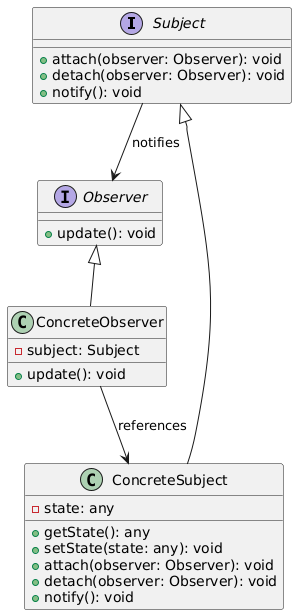
\includegraphics[width=0.47\textwidth]{images/oberver_gen.png} % Adjust width as needed
    \caption{Observer Pattern UML Class Diagram}
    \label{fig:example}
\end{figure}
\begin{figure}[h]
    \centering
    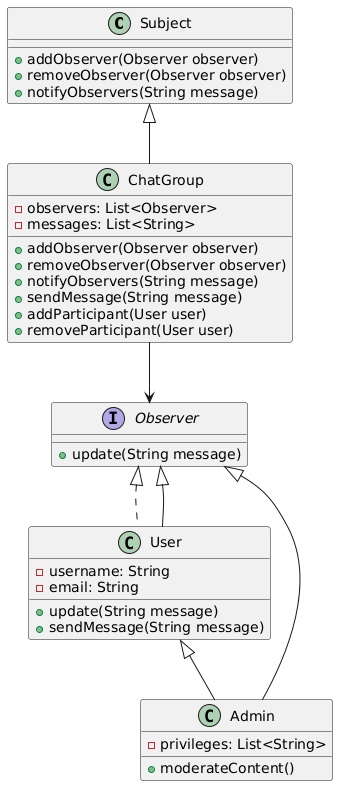
\includegraphics[width=0.47\textwidth]{images/observer.png} % Adjust width as needed
    \caption{Opberver Pattern for our Messinger Application}
    \label{fig:example}
\end{figure}

\chapter{UML Sequence diagrams}
\begin{figure}[h]
    \centering
    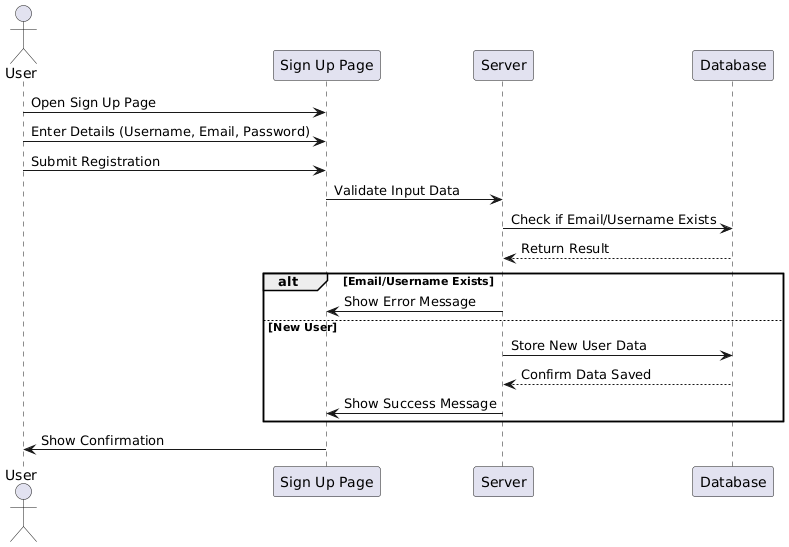
\includegraphics[width=0.7\textwidth]{images/register.png} % Adjust width as needed
    \caption{Register Sequence Diagram}
    \label{fig:example}
\end{figure}
\begin{longtable}{|c|p{10cm}|}
    \hline
    \textbf{Interactions} & \textbf{ Description} \\
    \hline
     Interaction1 & User opens the sign-up page. \\
    \hline
    Interaction2 & User enters registration details (username, email, password). \\
    \hline
    Interaction3 & User submits the registration form. \\
    \hline
    Interaction4 & Server validates input data. \\
    \hline
    Interaction5 & Server checks database for existing email/username. \\
    \hline
    Interaction6 & If email/username exists, an error message is shown. Otherwise, the server stores the new user data. \\
    \hline
    Interaction7 & Database confirms user registration. \\
    \hline
    Interaction8 & Server sends a success message to the sign-up page. \\
    \hline
    Interaction9 & User receives a confirmation message. \\
    \hline
\end{longtable}
\newpage

\begin{figure}[h]
    \centering
    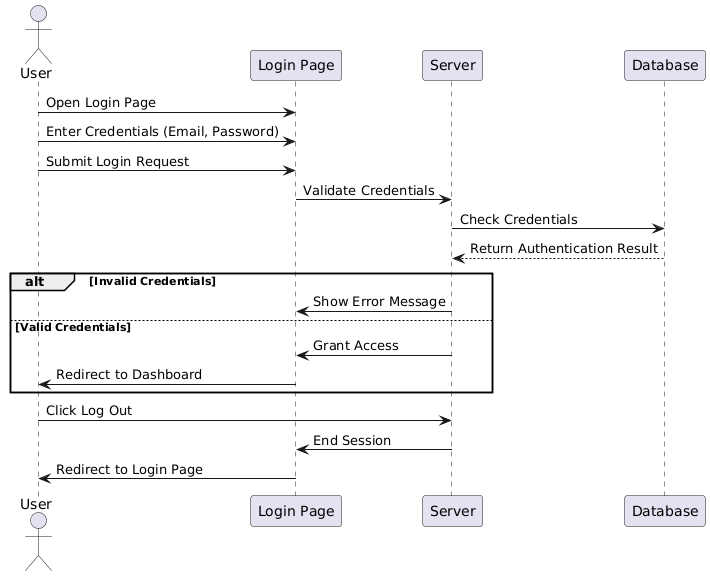
\includegraphics[width=0.7\textwidth]{images/login_out.png} % Adjust width as needed
    \caption{Log In/Out Sequence Diagram}
    \label{fig:example}
\end{figure}


\begin{longtable}{|c|p{10cm}|}
    \hline
    \textbf{Interactions} & \textbf{Description} \\
    \hline
    Interaction1 & User opens the login page. \\
    \hline
    Interaction2 & User enters login credentials (email, password). \\
    \hline
    Interaction3 & User submits the login request. \\
    \hline
    Interaction4 & Server validates the provided credentials. \\
    \hline
    Interaction5 & Server checks credentials in the database. \\
    \hline
    Interaction6 & Database returns authentication result. \\
    \hline
    Interaction7 & If credentials are invalid, an error message is displayed. Otherwise, the server grants access. \\
    \hline
    Interaction8 & If login is successful, user is redirected to the dashboard. \\
    \hline
    Interaction9 & User clicks log out. \\
    \hline
    Interaction10 & Server ends the user session. \\
    \hline
    Interaction11 & User is redirected to the login page. \\
    \hline
\end{longtable}
\newpage

\begin{figure}[h]
    \centering
    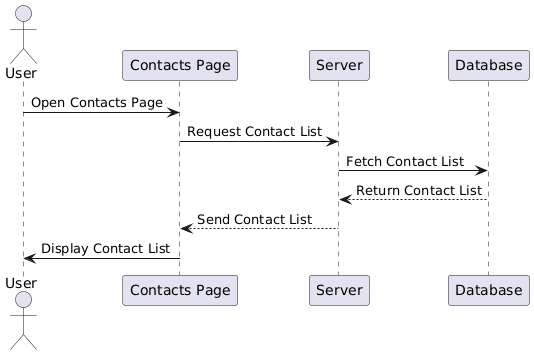
\includegraphics[width=0.7\textwidth]{images/view_contact_list.png} % Adjust width as needed
    \caption{View Contact List Sequence Diagram}
    \label{fig:example}
\end{figure}


\begin{longtable}{|c|p{10cm}|}
    \hline
    \textbf{Interactions} & \textbf{Description} \\
    \hline
    Interaction1 & User opens the contacts page. \\
    \hline
    Interaction2 & Contacts page requests the contact list from the server. \\
    \hline
    Interaction3 & Server fetches the contact list from the database. \\
    \hline
    Interaction4 & Database returns the contact list to the server. \\
    \hline
    Interaction5 & Server sends the contact list to the contacts page. \\
    \hline
    Interaction6 & Contacts page displays the contact list to the user. \\
    \hline
\end{longtable}
\newpage
\begin{figure}[h]
    \centering
    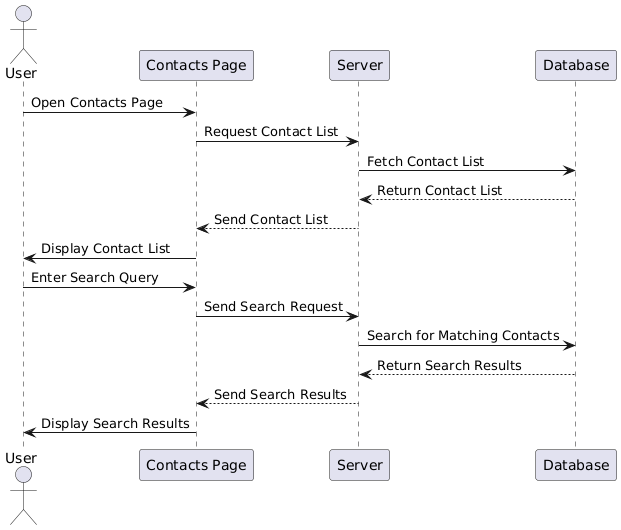
\includegraphics[width=0.7\textwidth]{images/search_contacts.png} % Adjust width as needed
    \caption{Search Contacts Sequence Diagram}
    \label{fig:example}
\end{figure}


\begin{longtable}{|c|p{10cm}|}
    \hline
    \textbf{Interactions} & \textbf{Description} \\
    \hline
    Interaction1 & User opens the contacts page. \\
    \hline
    Interaction2 & Contacts page requests the contact list from the server. \\
    \hline
    Interaction3 & Server fetches the contact list from the database. \\
    \hline
    Interaction4 & Database returns the contact list to the server. \\
    \hline
    Interaction5 & Server sends the contact list to the contacts page. \\
    \hline
    Interaction6 & Contacts page displays the contact list to the user. \\
    \hline
    Interaction7 & User enters a search query. \\
    \hline
    Interaction8 & Contacts page sends the search request to the server. \\
    \hline
    Interaction9 & Server searches for matching contacts in the database. \\
    \hline
    Interaction10 & Database returns the search results to the server. \\
    \hline
    Interaction11 & Server sends the search results to the contacts page. \\
    \hline
    Interaction12 & Contacts page displays the search results to the user. \\
    \hline
\end{longtable}
\newpage
\begin{figure}[h]
    \centering
    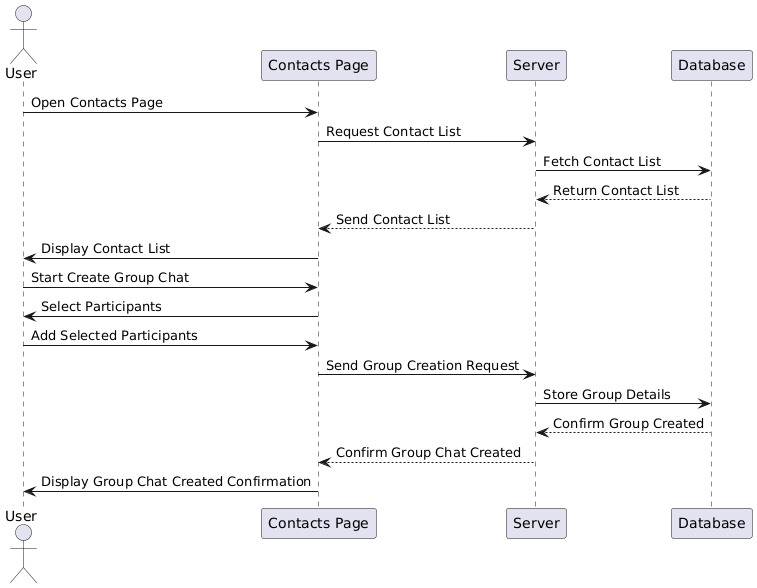
\includegraphics[width=0.7\textwidth]{images/create_grup.png} % Adjust width as needed
    \caption{Create Grup Chat Sequence Diagram}
    \label{fig:example}
\end{figure}


\begin{longtable}{|c|p{10cm}|}
    \hline
    \textbf{Interactions} & \textbf{Description} \\
    \hline
    Interaction1 & User opens the contacts page. \\
    \hline
    Interaction2 & Contacts page requests the contact list from the server. \\
    \hline
    Interaction3 & Server fetches the contact list from the database and returns it. \\
    \hline
    Interaction4 & Contacts page displays the contact list to the user. \\
    \hline
    Interaction5 & User starts the create group chat process. \\
    \hline
    Interaction6 & User selects participants for the group. \\
    \hline
    Interaction7 & Contacts page sends the group creation request to the server. \\
    \hline
    Interaction8 & Server stores the group details in the database. \\
    \hline
    Interaction9 & Contacts page displays the group chat creation confirmation to the user. \\
    \hline
\end{longtable}
\newpage

\begin{figure}[h]
    \centering
    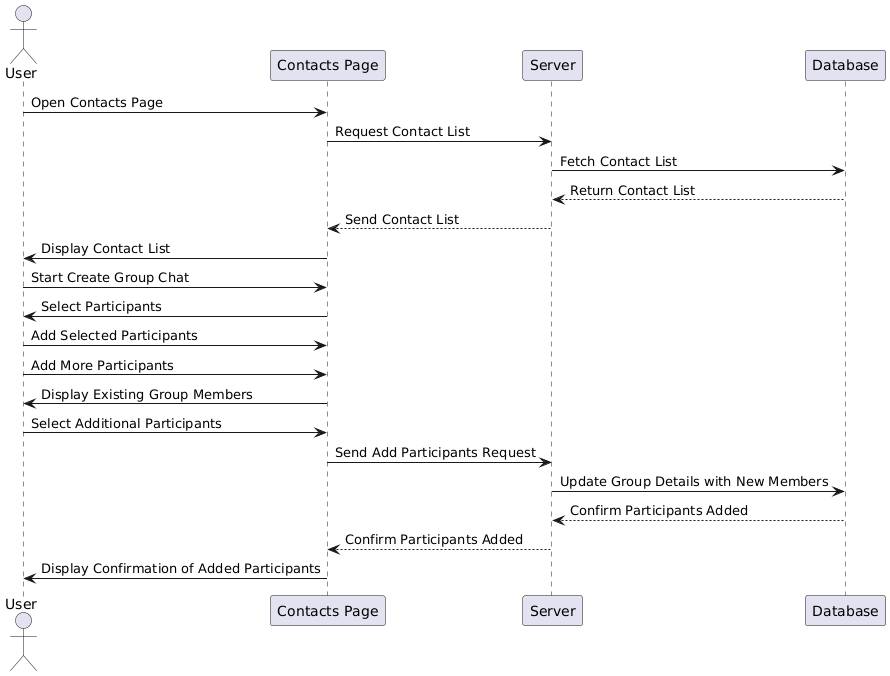
\includegraphics[width=0.7\textwidth]{images/add_to_grup.png} % Adjust width as needed
    \caption{Add Participants to Group Sequence Diagram}
    \label{fig:example}
\end{figure}


\begin{longtable}{|c|p{10cm}|}
    \hline
    \textbf{Interactions} & \textbf{Description} \\
    \hline
    Interaction1 & User opens the contacts page. \\
    \hline
    Interaction2 & Contacts page requests the contact list from the server. \\
    \hline
    Interaction3 & Server fetches the contact list from the database and returns it. \\
    \hline
    Interaction4 & Contacts page displays the contact list to the user. \\
    \hline
    Interaction5 & User starts the create group chat process. \\
    \hline
    Interaction6 & User selects participants and adds them to the group. \\
    \hline
    Interaction7 & User initiates adding more participants to an existing group. \\
    \hline
    Interaction8 & Contacts page displays the existing group members to the user. \\
    \hline
    Interaction9 & User selects additional participants for the group. \\
    \hline
    Interaction10 & Contacts page sends the add participants request to the server. \\
    \hline
    Interaction11 & Server updates the group details with the new members in the database. \\
    \hline
    Interaction12 & Server confirms that the participants were successfully added. \\
    \hline
    Interaction13 & Contacts page displays the confirmation of added participants to the user. \\
    \hline
\end{longtable}
\newpage

\begin{figure}[h]
    \centering
    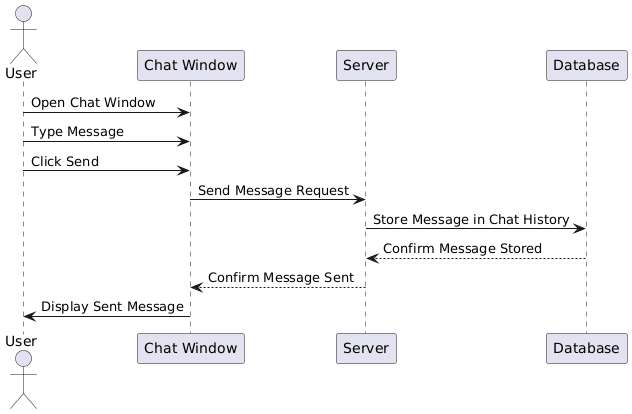
\includegraphics[width=0.7\textwidth]{images/send_message.png} % Adjust width as needed
    \caption{Send Message Sequence Diagram}
    \label{fig:example}
\end{figure}


\begin{longtable}{|c|p{10cm}|}
    \hline
    \textbf{Interactions} & \textbf{Description} \\
    \hline
    Interaction1 & User opens the chat window. \\
    \hline
    Interaction2 & User types a message. \\
    \hline
    Interaction3 & User clicks send to submit the message. \\
    \hline
    Interaction4 & Chat window sends the message request to the server. \\
    \hline
    Interaction5 & Server stores the message in the database. \\
    \hline
    Interaction6 & Database confirms the message has been stored. \\
    \hline
    Interaction7 & Server confirms the message has been sent to the chat window. \\
    \hline
    Interaction8 & Chat window displays the sent message to the user. \\
    \hline
\end{longtable}
\newpage

\begin{figure}[h]
    \centering
    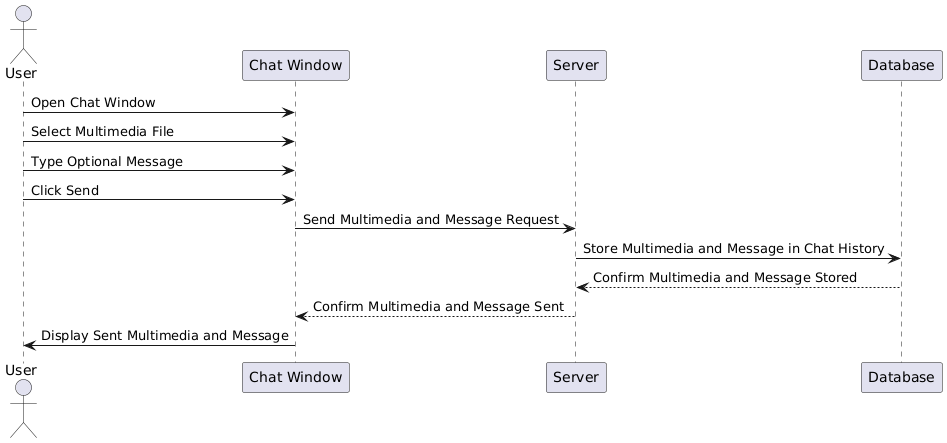
\includegraphics[width=0.7\textwidth]{images/send_multimedia.png} % Adjust width as needed
    \caption{Send Multimedia Sequence Diagram}
    \label{fig:example}
\end{figure}


\begin{longtable}{|c|p{10cm}|}
    \hline
    \textbf{Interactions} & \textbf{Description} \\
    \hline
    Interaction1 & User opens the chat window. \\
    \hline
    Interaction2 & User selects a multimedia file. \\
    \hline
    Interaction3 & User types an optional message. \\
    \hline
    Interaction4 & User clicks send to submit the multimedia and message. \\
    \hline
    Interaction5 & Chat window sends the multimedia and message request to the server. \\
    \hline
    Interaction6 & Server stores the multimedia and message in the database. \\
    \hline
    Interaction7 & Database confirms the multimedia and message have been stored. \\
    \hline
    Interaction8 & Server confirms the multimedia and message have been sent to the chat window. \\
    \hline
    Interaction9 & Chat window displays the sent multimedia and message to the user. \\
    \hline
\end{longtable}
\newpage
\begin{figure}[h]
    \centering
    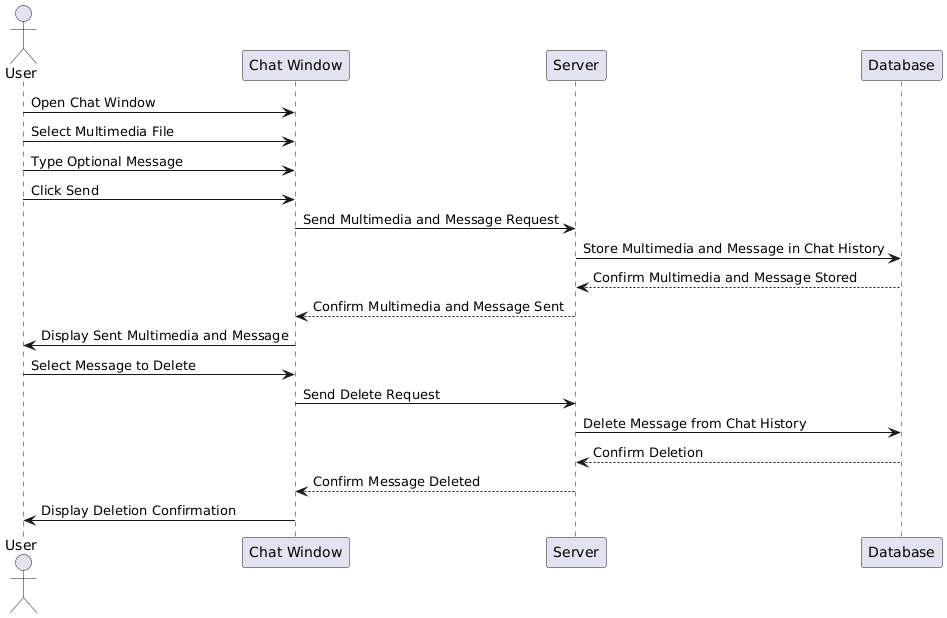
\includegraphics[width=0.7\textwidth]{images/de;ete_message.png} % Adjust width as needed
    \caption{Delete Message Sequence Diagram}
    \label{fig:example}
\end{figure}


\begin{longtable}{|c|p{10cm}|}
    \hline
    \textbf{Interactions} & \textbf{Description} \\
    \hline
    Interaction1 & User opens the chat window. \\
    \hline
    Interaction2 & User selects a multimedia file (optional step before sending a message). \\
    \hline
    Interaction3 & User types an optional message and clicks send. \\
    \hline
    Interaction4 & Chat window sends the multimedia and message request to the server. \\
    \hline
    Interaction5 & Server stores the multimedia and message in the database. \\
    \hline
    Interaction6 & Database confirms the multimedia and message have been stored. \\
    \hline
    Interaction7 & Chat window displays the sent multimedia and message to the user. \\
    \hline
    Interaction8 & User selects a message to delete. \\
    \hline
    Interaction9 & Chat window sends the delete request to the server. \\
    \hline
    Interaction10 & Server deletes the message from the chat history in the database. \\
    \hline
    Interaction11 & Database confirms the message has been deleted. \\
    \hline
    Interaction12 & Chat window displays the deletion confirmation to the user. \\
    \hline
\end{longtable}
\newpage
\begin{figure}[h]
    \centering
    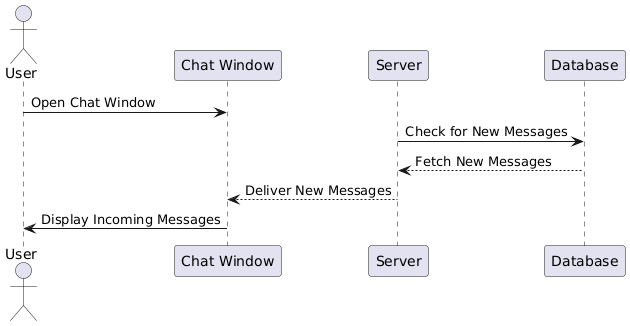
\includegraphics[width=0.7\textwidth]{images/recive_message.png} % Adjust width as needed
    \caption{Recive Message Sequence Diagram}
    \label{fig:example}
\end{figure}


\begin{longtable}{|c|p{10cm}|}
    \hline
    \textbf{Interactions} & \textbf{Description} \\
    \hline
    Interaction1 & User opens the chat window. \\
    \hline
    Interaction2 & Server checks the database for new messages. \\
    \hline
    Interaction3 & Database fetches the new messages and sends them to the server. \\
    \hline
    Interaction4 & Server delivers the new messages to the chat window. \\
    \hline
    Interaction5 & Chat window displays the incoming messages to the user. \\
    \hline
\end{longtable}
\newpage

\begin{figure}[h]
    \centering
    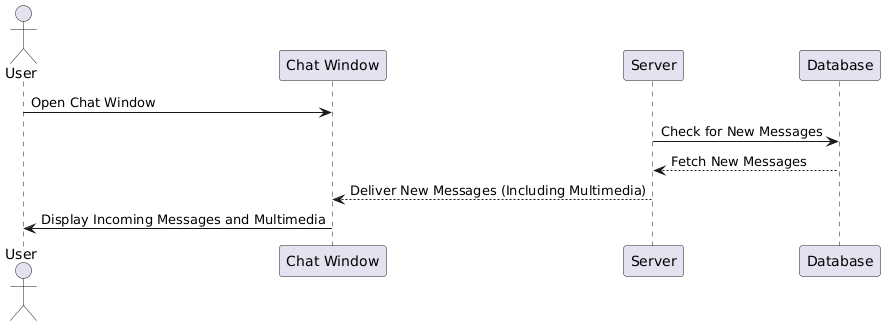
\includegraphics[width=0.7\textwidth]{images/recive_multimedia.png} % Adjust width as needed
    \caption{Receive Multimedia Sequence Diagram}
    \label{fig:example}
\end{figure}


\begin{longtable}{|c|p{10cm}|}
    \hline
    \textbf{Interactions} & \textbf{Description} \\
    \hline
    Interaction1 & User opens the chat window. \\
    \hline
    Interaction2 & Server checks the database for new messages. \\
    \hline
    Interaction3 & Database fetches the new messages, including multimedia, and sends them to the server. \\
    \hline
    Interaction4 & Server delivers the new messages, including multimedia, to the chat window. \\
    \hline
    Interaction5 & Chat window displays the incoming messages and multimedia to the user. \\
    \hline
\end{longtable}
\newpage

\begin{figure}[h]
    \centering
    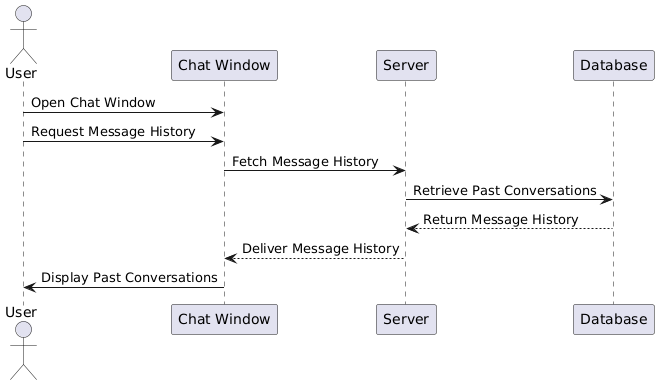
\includegraphics[width=0.7\textwidth]{images/chat_history.png} % Adjust width as needed
    \caption{View Chat History Sequence Diagram}
    \label{fig:example}
\end{figure}


\begin{longtable}{|c|p{10cm}|}
    \hline
    \textbf{Interactions} & \textbf{Description} \\
    \hline
    Interaction1 & User opens the chat window. \\
    \hline
    Interaction2 & User requests message history. \\
    \hline
    Interaction3 & Chat window sends a request to the server to fetch message history. \\
    \hline
    Interaction4 & Server retrieves past conversations from the database. \\
    \hline
    Interaction5 & Database returns the message history to the server. \\
    \hline
    Interaction6 & Server delivers the message history to the chat window. \\
    \hline
    Interaction7 & Chat window displays past conversations to the user. \\
    \hline
\end{longtable}
\newpage

\begin{figure}[h]
    \centering
    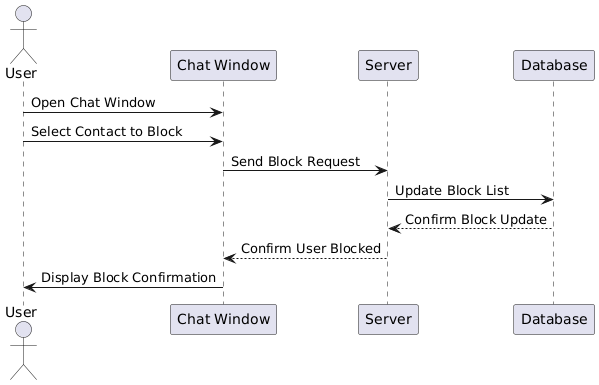
\includegraphics[width=0.7\textwidth]{images/block_user.png} % Adjust width as needed
    \caption{Block User Sequence Diagram}
    \label{fig:example}
\end{figure}


\begin{longtable}{|c|p{10cm}|}
    \hline
    \textbf{Interactions} & \textbf{Description} \\
    \hline
    Interaction1 & User opens the chat window. \\
    \hline
    Interaction2 & User selects a contact to block. \\
    \hline
    Interaction3 & Chat window sends the block request to the server. \\
    \hline
    Interaction4 & Server updates the block list in the database. \\
    \hline
    Interaction5 & Database confirms the block list update. \\
    \hline
    Interaction6 & Server confirms the contact has been blocked. \\
    \hline
    Interaction7 & Chat window displays the block confirmation to the user. \\
    \hline
\end{longtable}
\newpage

\begin{figure}[h]
    \centering
    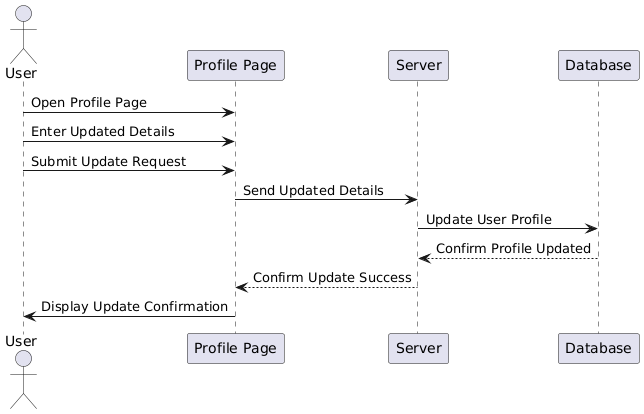
\includegraphics[width=0.7\textwidth]{images/edit_profile.png} % Adjust width as needed
    \caption{Edit Profile Sequence Diagram}
    \label{fig:example}
\end{figure}


\begin{longtable}{|c|p{10cm}|}
    \hline
    \textbf{Interactions} & \textbf{Description} \\
    \hline
    Interaction1 & User opens the profile page. \\
    \hline
    Interaction2 & User enters updated profile details. \\
    \hline
    Interaction3 & User submits the update request. \\
    \hline
    Interaction4 & Profile page sends the updated details to the server. \\
    \hline
    Interaction5 & Server updates the user profile in the database. \\
    \hline
    Interaction6 & Database confirms that the profile has been updated. \\
    \hline
    Interaction7 & Server confirms the successful update to the profile page. \\
    \hline
    Interaction8 & Profile page displays the update confirmation to the user. \\
    \hline
\end{longtable}

\newpage
\begin{figure}[h]
    \centering
    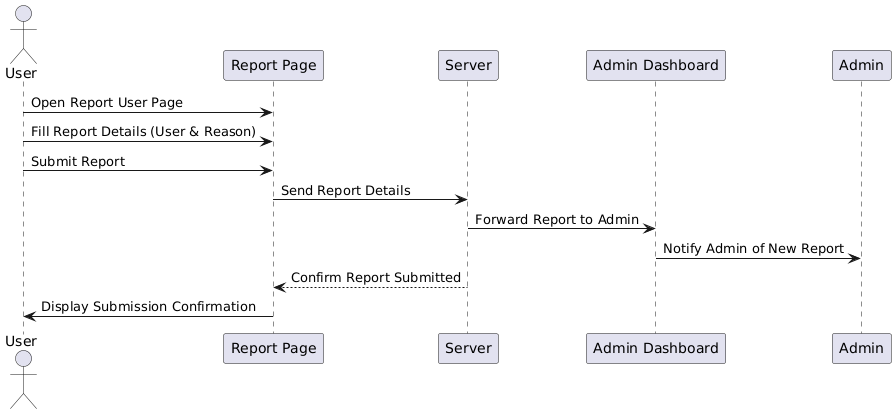
\includegraphics[width=0.7\textwidth]{images/report_user.png} % Adjust width as needed
    \caption{Report User Sequence Diagram}
    \label{fig:example}
\end{figure}


\begin{longtable}{|c|p{10cm}|}
    \hline
    \textbf{Interactions} & \textbf{Description} \\
    \hline
    Interaction1 & User opens the report user page. \\
    \hline
    Interaction2 & User fills in report details, including the user to report and the reason. \\
    \hline
    Interaction3 & User submits the report. \\
    \hline
    Interaction4 & Report page sends the report details to the server. \\
    \hline
    Interaction5 & Server forwards the report to the admin dashboard. \\
    \hline
    Interaction6 & Admin dashboard notifies the admin of the new report. \\
    \hline
    Interaction7 & Server confirms the report submission to the report page. \\
    \hline
    Interaction8 & Report page displays the submission confirmation to the user. \\
    \hline
\end{longtable}

\chapter{Application architecture }

The architecture of the messenger application consists of five main components: User Devices, Server Application, Communication Type (Wireless), Central Database, and Frontend.This architecture ensures efficient communication, scalability, and reliable data storage, while maintaining a seamless user experience.
\thispagestyle{pagestyle}
\begin{figure}[h]
    \centering
    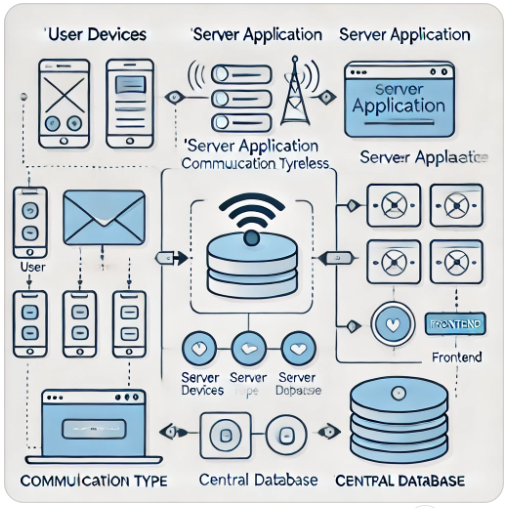
\includegraphics[width=0.47\textwidth]{images/arhitecture.PNG} % Adjust width as needed
    \caption{Aplication Arhitecture}
    \label{fig:example}
\end{figure}


User Devices are end-user devices like smartphones, tablets, or computers that serve as the primary interface for interacting with the messenger application. They enable users to send messages, receive notifications, and perform various interactions, acting as the entry and exit point for user activity. These devices communicate wirelessly with the Server Application via Wi-Fi, mobile data, or other network protocols.


Server Application is the core of the messenger service, responsible for processing and managing all system operations. It handles requests from user devices, routes messages to the correct recipients, and implements essential business logic such as message encryption, and validation. The server directly communicates with user devices to send and receive data, interacts with the Central Database for storing and retrieving persistent data, and provides data and functionality to the Frontend.


Communication Type represents the network used for transferring data between User Devices and the Server Application. It enables real-time communication between users via protocols such as Wi-Fi, 4G/5G, ensuring a stable connection for delivering messages and notifications. This wireless communication seamlessly connects User Devices with the Server Application.



Central Database is a centralized storage system that manages all persistent data for the application, including messages, user profiles, settings, and other critical information. It ensures data integrity and facilitates querying for message history or user-related details. The Server Application interacts with the database to fetch or store data during message operations or user requests.


Frontend is the UI(User Interface), user-facing part of the system, offering a web-based interface for users or administrators to manage application settings, monitor activity, and send or receive messages. It presents data processed by the Server Application in a user-friendly format and directly interacts with the server to display or retrieve information.